\documentclass{standalone}
\usepackage{tikz,bm}
\begin{document}
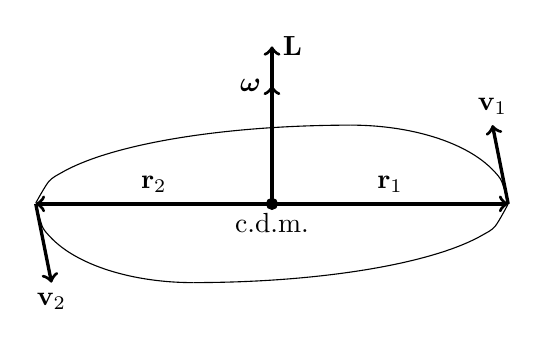
\begin{tikzpicture}[scale=2]
    \draw[-]plot[smooth, domain=-1.5:-0.5](\x,{-0.5*(1-(\x+0.5)^2)^0.5});
    \draw[-]plot[smooth, domain=0.5:1.5](\x,{0.5*(1-(\x-0.5)^2)^0.5});
    \draw[-]plot[smooth, domain=0.5:-1.5](\x,{0.25*(4-(\x-0.5)^2)^0.5});
    \draw[-]plot[smooth, domain=1.5:-0.5](\x,{-0.25*(4-(\x+0.5)^2)^0.5});

    
    \draw[->,very thick](0,0)--(0,0.75)node[left]{$\boldsymbol{\omega}$};
    \draw[->, very thick](0,0)--(0,1)node[right]{$\mathbf{L}$};
    \filldraw[black](0,0)circle(1pt);
    \node[below]at(0,0){$\mathrm{c.d.m.}$};


    \draw[->, very thick](0,0)--(1.5,0)node[midway, above]{$\mathbf{r}_1$};
    \draw[->, very thick](0,0)--(-1.5,0)node[midway, above]{$\mathbf{r}_2$};    

    \draw[->, very thick](1.5,0)--(1.4,0.5)node[above]{$\mathbf{v}_1$};    
    \draw[->, very thick](-1.5,0)--(-1.4,-0.5)node[below]{$\mathbf{v}_2$};
\end{tikzpicture}
\end{document}